\documentclass{article}

% \usepackage[utf8]{inputenc} %Stationær ÆØÅ
\usepackage[ansinew]{inputenc} %Bærbar ÆØÅ?

%\usepackage{url} % Allows hyperlinks
\usepackage[hyphens]{url} %URLs
\usepackage{graphicx} % Allows figures
% \usepackage{etoolbox} %for configuration of sloppy

%Section style
\usepackage{xcolor}

\definecolor{secnum}{RGB}{102,102,102} 

\makeatletter
    \def\@seccntformat#1{\llap{\color{secnum}\csname the#1\endcsname\hskip 16pt}}
\makeatother
%end section style

% \apptocmd{\sloppy}{\hbadness 10000\relax}{}{} %adds hbadness to sloppy
\setlength{\paperheight}{297mm} %Sets the page to an A4
\setlength{\paperwidth}{210mm}	%Sets the page to an A4

\begin{document}

\begin{titlepage}
\begin{center}
\textsc{\Large IT Sikkerhed}\\[0.5cm]
\textsc{OPGAVE B: Sikkerhedsanalyse af sociale medier}\\[0.5cm]
\vspace{2 cm}
\begin{tabular}{ll}
Kasper Passov & pvx884\\
\end{tabular}
\end{center}
\vspace{5 cm}
\newpage
\tableofcontents
\end{titlepage}

\section{Resumé af systemet}
Facebook, Twitter, LinkedIn og Internt Yammer til internt og ekstern kommunikere
Deler systemerne op i Eksterne (Facebook, Twitter og LinkedIn) Kun kommunikations ansatte der har adgang 
og interne (Yammer) Alle medarbejdere har en konto.


\section{Aktiver}
\subsection{Externe systemer}
Administrative kontoer skal beskyttes. Mulighed for informationsdeling skal holdes åben.

\subsection{Interne systemer}
Informationen på det interne system Yammer skal beskyttes fra udekommende. Ansatte skal have nem og hurtig adgang til information, gerne hvor som helst og når som helst. Ansattes information skal beskyttes. Ansattes brugere og passwords. 

\subsection{Begrundelse for aktiver}

\section{Sikkerhedsmål}



\section{Trusselsaktører}

Internt:
Hackere
(Utilfredse ansatte)


Eksternt:
Konkurenter
Hackere
(Utilfredse ansatte)

\section{Trusler}

Internt:

Udbyder leaker passwords
Ansatte mister passwords

Eksternt:

Udbyder Leaked passwords
Ansatte mister passwords

\subsection{Relevante angreb}
\subsubsection{AP's Twitter-konto}

\begin{figure}
  \begin{center}
    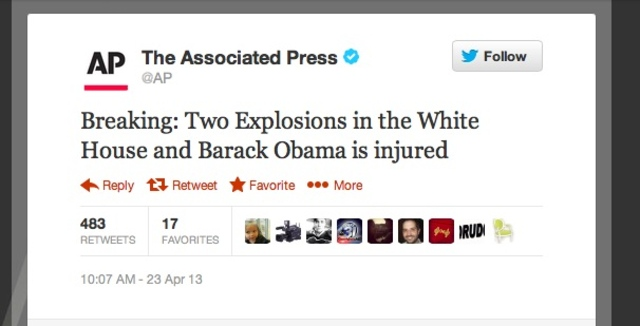
\includegraphics[width=0.6\textwidth]{../Pictures/APTweet.jpg}
  \end{center}
  \caption{Tweeten fra hackeren over nyhedsbureauet Associated Press \cite{APTweetSource}}
\end{figure}

\paragraph{Angreb}
\url{www.guardian.co.uk/business/2013/apr/23/ap-tweet-hack-wall-street-freefall Her er historien}
\paragraph{Relevans for BIOmedix}

Et sådan angreb kan fjerne tilid og lade konkurrenter samt ondsindede hacker sprede misinformation in BIOmedix navn 
\subsubsection{LinkedIn password-lækage}

\paragraph{Angreb}
\url{arstechnica.com/security/2012/06/8-million-leaked-passwords-connected-to-linkedin/}
\paragraph{Relevans for BIOmedix}

Et stort leak af passwords fra en sådan side kunne betyde alle BIOmedix' sociale medie sider ville være usikre, hvis det samme password var brugt overalt. Kig information igennem for ændringer, og skift password. SØRG FOR DER ER FORSKELLIGE PASSWORDS TIL ALLE SIDER DER BRUGER SAMME MAIL! 

\section{Sårbarheder}



\section{Modforanstaltninger}

Password styrke og brug

\section{Risici}



\section{Foreslåede modforanstaltninger}



\section{Konklusion}


\newpage
\begin{thebibliography}{100}


\bibitem{APTweetSource}
\url{www.businessinsider.com/ap-hacked-obama-injured-white-house-explosions-2013-4}
\bibitem{APTweetStory} 
\url{www.guardian.co.uk/business/2013/apr/23/ap-tweet-hack-wall-street-freefall}
\end{thebibliography}
\end{document}
